  
  
  \frame{
  \frametitle{What are \emph{containers} and \emph{Virtual Machines}?}
  \begin{columns}[T] % align columns
  \begin{column}{.80\textwidth}
  	\begin{itemize}
   		\item Containers and Virtual Machines (VM) are similar in their goals: 
\begin{enumerate}   		
   		\item \emph{\color{NavyBlue}to provide analysis \textbf{portability} isolating an application  into a self-contained unit that can run anywhere};\vspace{0.3cm}
   		\item \emph{\color{NavyBlue}to provide analysis \textbf{reproducibility} freezing the version of  tools and libraries used.}
   		\end{enumerate}
   		\vspace{0.3cm}
   		\item  They remove the need for physical hardware, allowing for more efficient use of computing resources, both in terms of energy consumption and cost effectiveness;\vspace{0.3cm}
   		\item 	The main difference between containers and VMs is in their architectural approach.
   		\end{itemize}\vspace{0.3cm}
   \end{column}%
   \hfill%
   \begin{column}{0.20\textwidth}
     	\begin{center}
  			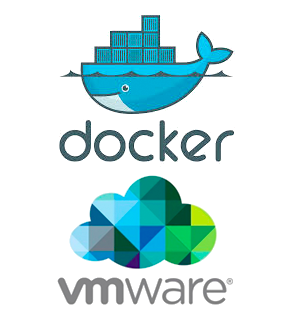
\includegraphics[width=1.15\columnwidth]{./Figure/DockerVSVM}\\
  		\end{center}
   \end{column}%
   \end{columns}
  } 



 \frame{
  \frametitle {Virtual Machines}
  
  \begin{columns}[T] % align columns
  \begin{column}{.55\textwidth}
  	\begin{itemize}
 		\item A VM is essentially an emulation of a real computer (i.e.\emph{ \color{NavyBlue} guest machine}) that executes programs like a real computer;\vspace{0.3cm}
 
 		\item  VMs run on top of a physical machine (i.e.\emph{\color{NavyBlue} host machine}) using a \emph{\color{NavyBlue}hypervisor};\vspace{0.3cm}
 
 		\item A {\color{NavyBlue}hypervisor} is a piece of software, firmware, or hardware;\vspace{0.3cm}
 		
 		\item A {\color{NavyBlue}guest machine} contains:
		
		\begin{itemize}	 		
 		
 		 \item both the application and whatever it needs to run that application (e.g. system binaries and libraries). 
 	
 	    \item a virtualized hardware stack including virtualized network adapters, storage, CPU \dots.
 	
 		\end{itemize}
 		
      	\end{itemize}
   \end{column}%
   \hfill%
   \begin{column}{0.45\textwidth}
     	\begin{center}
  			\includegraphics[width=1.00\columnwidth]{./Figure/VM}\\
  		\end{center}
   \end{column}%
   \end{columns}
  } 
  
  
  
  
  \frame{
  \frametitle {Containers}
  
  \begin{columns}[T] % align columns
  \begin{column}{.55\textwidth}
  	\begin{itemize}
 		\item Unlike a VM which provides hardware virtualization, a container provides operating-system-level virtualization by abstracting the \emph{\color{NavyBlue} user space};\vspace{0.3cm}
 
 		\item The main difference between containers and VMs is that containers \textbf{share} the host system's kernel with other containers.\vspace{0.3cm}
 
      	\end{itemize}
   \end{column}%
   \hfill%
   \begin{column}{0.45\textwidth}
     	\begin{center}
  			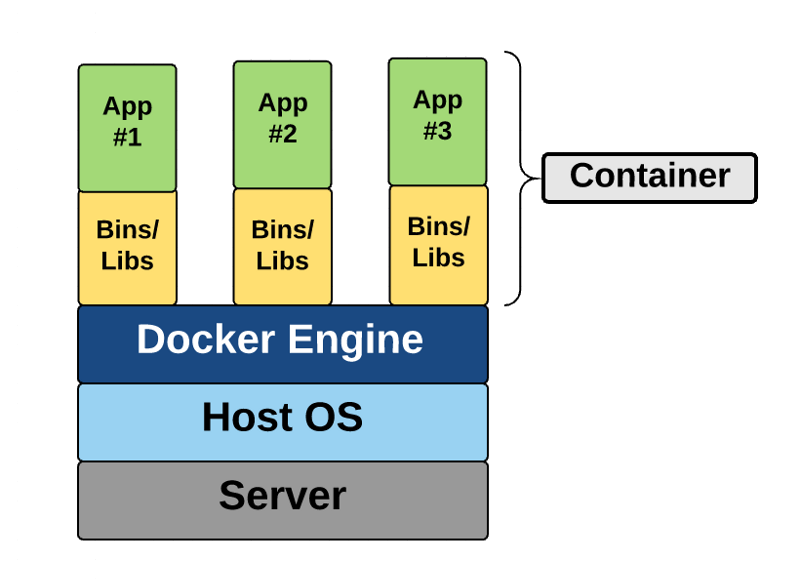
\includegraphics[width=1.05\columnwidth]{./Figure/Container}\\
  		\end{center}
   \end{column}%
   \end{columns}
  } 
  

 \frame{
  \frametitle {Containers VS VM}
  
  \begin{columns}[T] % align columns
  \begin{column}{.50\textwidth}
		\begin{center}
  			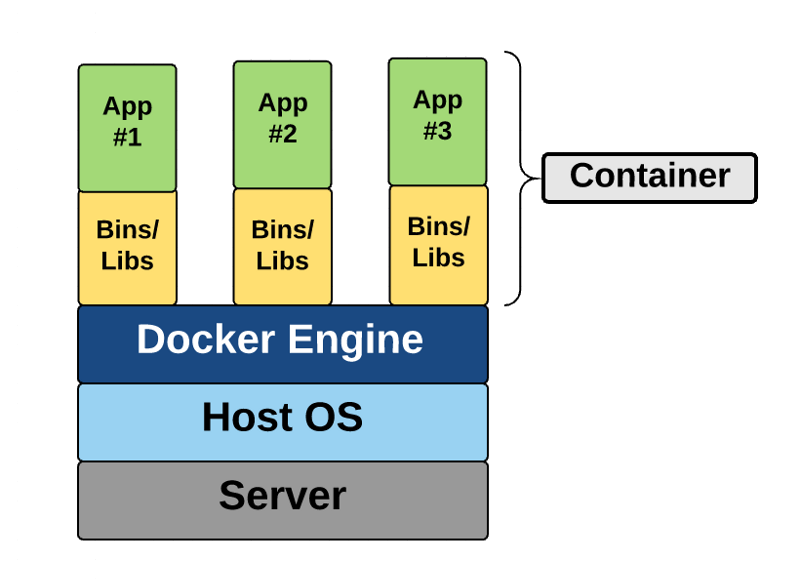
\includegraphics[width=1.00\columnwidth]{./Figure/Container}\\
  		\end{center}
   \end{column}%
   \hfill%
   \begin{column}{0.50\textwidth}
     	\begin{center}
  			\includegraphics[width=1.00\columnwidth]{./Figure/VM}\\
  		\end{center}
   \end{column}%
   \end{columns}
  } 

\frame{
  \frametitle {Containers VS VM}
 	\begin{center}
  			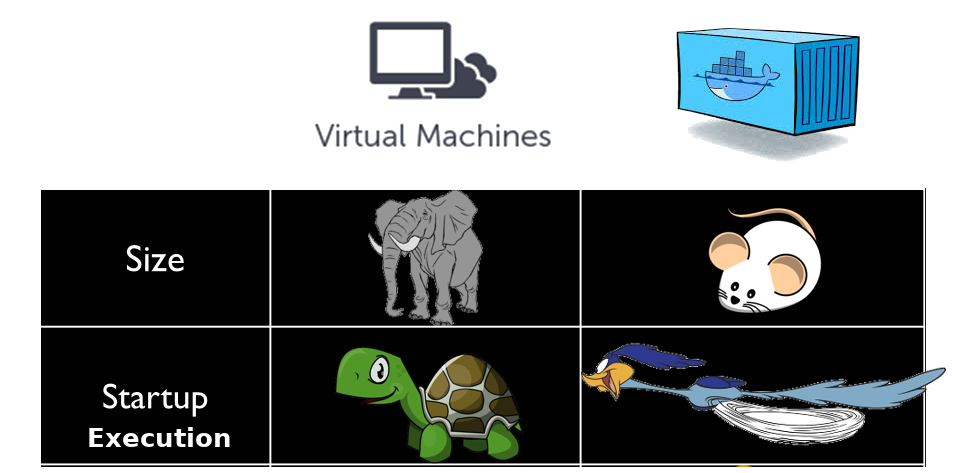
\includegraphics[width=0.90\columnwidth]{./Figure/ContainersVSVM}\\
  		\end{center}
  } 

\frame{
\frametitle{Docker container, VM and real server: a comparison}
In [1] a comparison among physical server, KVM, and Docker is reported.

     	\begin{center}
  			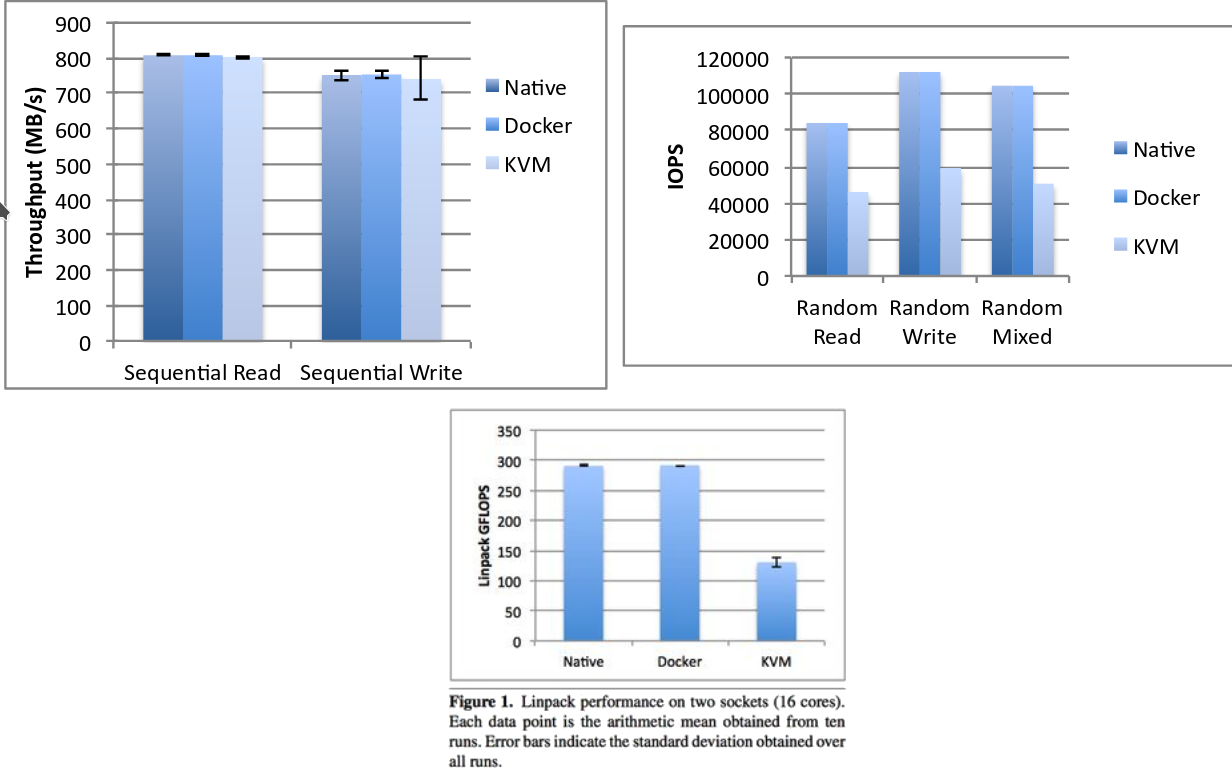
\includegraphics[width=0.90\columnwidth]{./Figure/benchmark}
  		\end{center}  
{\tiny
[1] W. Felter, A. Ferreira, R. Rajamony and J. Rubio, \emph{\textbf{An updated performance comparison of virtual machines and Linux containers}}, 2015 IEEE International Symposium on Performance Analysis of Systems and Software (ISPASS), Philadelphia, PA, 2015, pp. 171-172.

}
} 



\frame{
\frametitle{Computational Reproducibility Stack}

       	\begin{center}
  			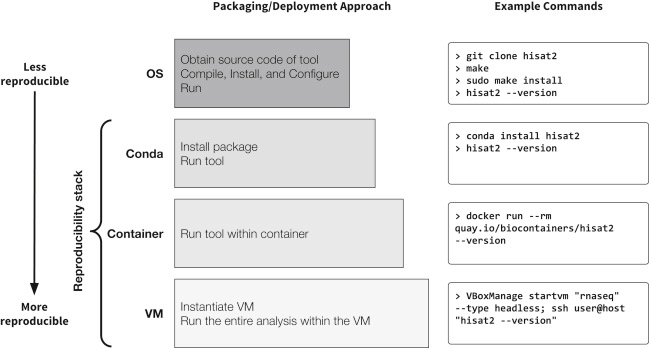
\includegraphics[width=0.9\columnwidth]{./Figure/stack}\\
  		\end{center}
}

 \frame{
  \frametitle {}
  \centerline{\Huge \color{NavyBlue} \textbf{\emph{Docker project}}}
       	\begin{center}
  			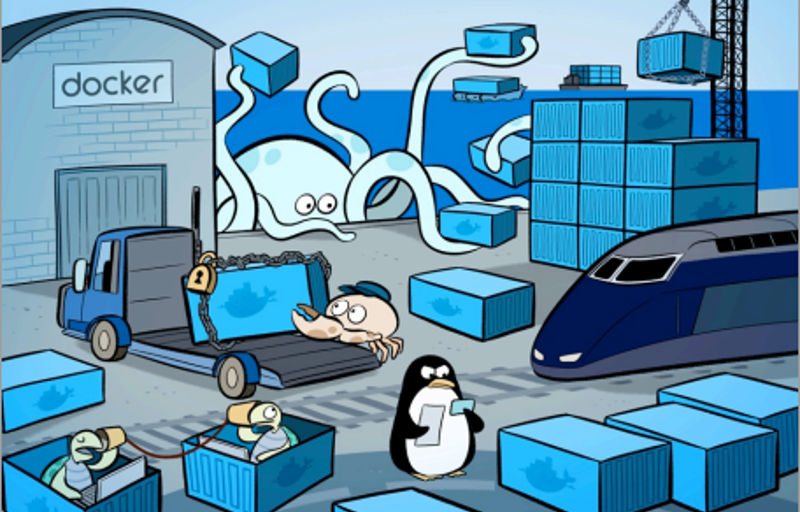
\includegraphics[width=0.8\columnwidth]{./Figure/basic}\\
  		\end{center}
}

  
  
 \frame{
  \frametitle {Docker project}
  
  
  
  \begin{columns}[T] % align columns
  \begin{column}{.55\textwidth}
  	\begin{itemize}
 		\item Docker is an open-source project based on Linux containers.
 	\vspace{0.3cm}
 		\item Others Linux container technologies include Solaris Zones, BSD jails, and LXC, which have been around for many years.
 		 	\vspace{0.3cm}	
      	\end{itemize}
   \end{column}%
   \hfill%
   \begin{column}{0.45\textwidth}
     	\begin{center}
  			
\includegraphics[width=1.05\columnwidth]{./Figure/Docker}\\
  		\end{center}
   \end{column}%
   \end{columns}
   \centerline{\Large \color{NavyBlue} \textbf{Why to use Docker??}}
  } 
  
  
  

 \frame{
  \frametitle {Why to use Docker?}
  
    \begin{columns}[T] % align columns
  \begin{column}{.65\textwidth}
  	\begin{itemize}
	\item  \textbf{\color{NavyBlue} Ease of use:} Docker has made it much easier for anyone to take advantage of containers in order to quickly build and test portable applications; \vspace{0.3cm}	
	
	\item  \textbf{\color{NavyBlue} Speed:} Docker containers are very lightweight and fast.
	\vspace{0.3cm}	
	\item \textbf{\color{NavyBlue}Docker Hub:} Docker users also benefit from the increasingly rich repository of Docker Hub, which you can think of as an "app store for Docker images"; 
	\vspace{0.3cm}	
	\item \textbf{\color{NavyBlue}Modularity and Scalability:} Docker makes it easy to break out your application's functionality into individual containers.
  	\end{itemize}
   \end{column}%
   \hfill%
   \begin{column}{0.35\textwidth}
     	\begin{center}
  			
\includegraphics[width=1.05\columnwidth]{./Figure/Docker}\\
  		\end{center}
   \end{column}%
   \end{columns}
  } 
    
  

  \frame{
\frametitle{Docker basics} 
\vspace{0.2cm}
\begin{itemize}
\item \textbf{\color{NavyBlue}\emph{Image}} is an executable package that includes everything needed to run an application (i.e. its code,  libraries, environment variables, and configuration files);\vspace{0.2cm}
\item \textbf{\color{NavyBlue}\emph{Container}} is a run-time instance of an image;\vspace{0.2cm}
\item \textbf{\color{NavyBlue}\emph{Volume}} is used to  share files from the host machine to containers.
\end{itemize}
\vspace{0.2cm}
  \begin{center}
  			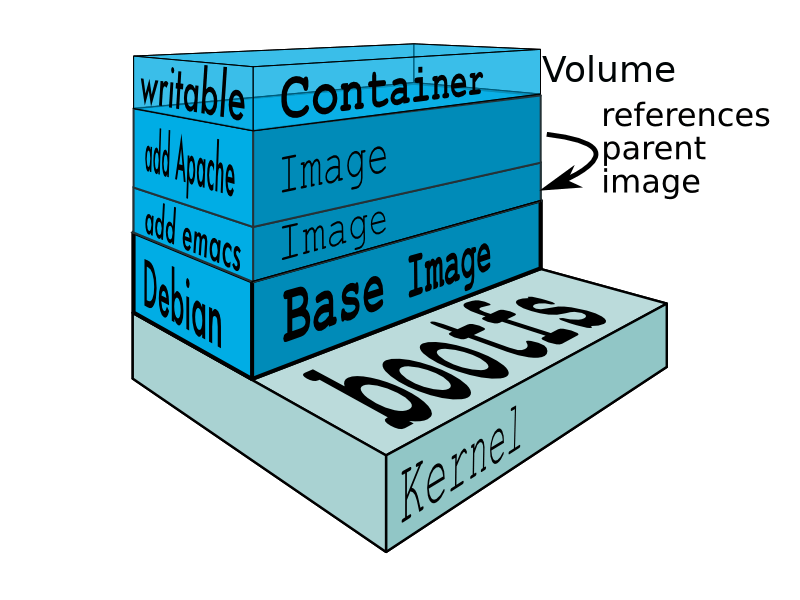
\includegraphics[width=0.55\columnwidth]{./Figure/exec}\\
  		\end{center} 

}

 \frame{
  \frametitle {Docker schema}
  
  
  
  \begin{columns}[T] % align columns
  \begin{column}{.55\textwidth}
  	\begin{itemize} 		
  	\item \textbf{\color{NavyBlue}Docker client:} provides an interface for users;
 	\vspace{0.2cm}
 		\item \textbf{\color{NavyBlue}Docker Host:} executes the commands sent to the Docker Client;\vspace{0.2cm}

 		\item \textbf{\color{NavyBlue}Docker Hub:} remove repository storing docker's images.
      	\end{itemize}
   \end{column}%
   \hfill%
   \begin{column}{0.45\textwidth}
     	\begin{center}
  			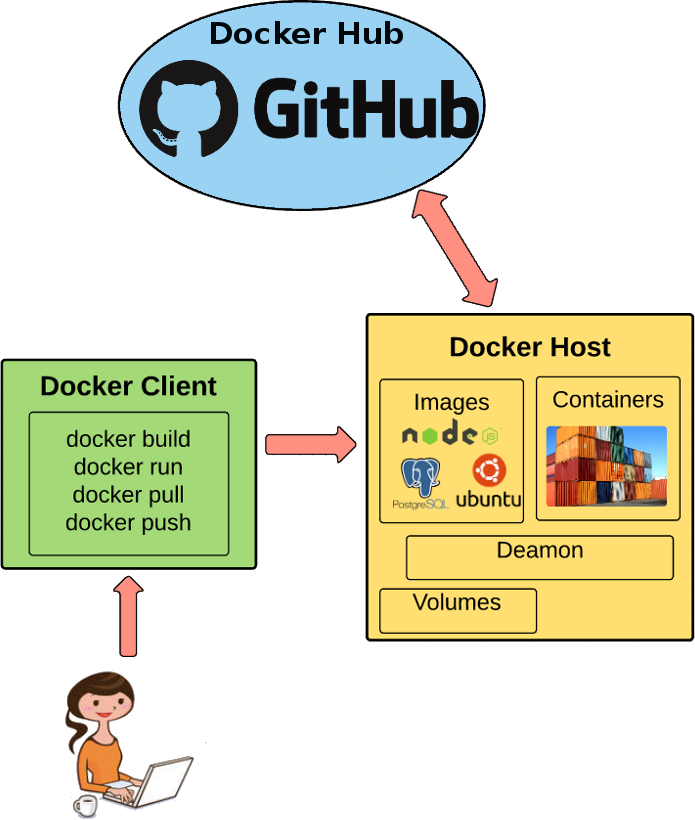
\includegraphics[width=0.95\columnwidth]{./Figure/DockerSchema}\\
  		\end{center}
   \end{column}%
   \end{columns}
  } 